\lecture{6}{9. April 2026}{Root Locus Method, I}

\section{The Root Locus Method} \label{sec:rlmethod}

\subsection{Introduction and Concepts}
For the unity-feedback system,
\begin{equation*}
  \frac{Y(s)}{R(s)} = \frac{KG(s)}{1 + KG(s)}
\end{equation*}
the closed-loop poles are the roots of the denominator, so they satisfy
\begin{equation*}
  1 + KG(s) = 0
.\end{equation*}
This equation is the characteristic equation.

So root locus means that we pick a value of $K$, solve $1 + KG(s) = 0$, plot the resulting closed-loop poles in the $s$-plane and then vary $K$ from 0 to $\infty$.
The curve traced by these poles is the root locus.

We can rewrite the above characteristic equation as
\begin{equation*}
  KG(s) = -1
\end{equation*}
which is useful because $-1$ has magnitude 1 and angle \ang{180} modulo \ang{360}.
This means we can split the condition into two parts:
\begin{align*}
  \left| KG(s) \right| &= 1 \\
  \angle KG(s) &= \ang{180} + k \ang{360} 
.\end{align*}
The key idea then is that changing $G$ changes the magnitude, but not the angle if $K > 0$.
So the angle condition tells where the root locus can exist and the magnitude condition tells which value of $K$ places a pole at that point.

\begin{exa}[Example system]
  We consider the example system on \Cref{fig:2ordersys} with open-loop transfer function
  \begin{equation*}
    G(s) = \frac{1}{s (s+2)}
  \end{equation*}
  and gain $K$, so
  \begin{equation*}
    KG(s) = \frac{K}{s(s+2)}
  .\end{equation*}
  Which means that the open-loop poles are at $s = 0$ and $s = -2$.
  There are no zeros.
  The two roots are where the root-locus branches start when $K = 0$.

  Using
  \begin{equation*}
    1 + KG(s) = 0 = 1+ \frac{K}{s(s+2)}
  \end{equation*}
  we multiply by $s(s+2)$ to get
  \begin{equation*}
    s(s+2) + K = 0
  \end{equation*}
  so
  \begin{equation*}
    s^2 + 2s + K = 0
  \end{equation*}
  which is the closed-loop characteristic equation.
  We can compare this to the standard second-order form
  \begin{equation*}
    s^2 + 2 \zeta \omega_n s + \omega_n^2 = 0
  .\end{equation*}
  Matching coefficients gives:
  \begin{equation*}
    2\zeta \omega_n = 2 \quad \text{and} \quad \omega_n^2 = K
  .\end{equation*}
  So
  \begin{equation*}
    \zeta \omega_n = 1, \qquad \omega_n = \sqrt{K}
  .\end{equation*}
  Which means
  \begin{equation*}
    \zeta = \frac{1}{\sqrt{K}}
  .\end{equation*}
  So as $K$ increases $\omega_n$ also increases, but $\zeta$ decreases.

  Solving
  \begin{equation*}
    s^2 + 2s + K = 0
  \end{equation*}
  gives
  \begin{equation*}
    s_{1,2 } = -1 \pm \sqrt{1 - K}
  .\end{equation*}
  When $0 < K < 1$, $\sqrt{1 - K}$ is real, so both poles are real.
  One will move rightward from $-2$ and one will move leftward from 0 approaching each other along the real axis.

  When $K = 1$ $s = -1$ so both poles meet at $-1$ which is the breakaway point.

  When $K > 1$, $\sqrt{1- K } = j \sqrt{K-1}$, so the poles are $s = -1 \pm j \sqrt{K - 1}$, from where they move vertically upward and downward, with constant real part $-1$. 

  Further, for this system
  \begin{equation*}
    KG(s) = \frac{K}{s(s+2)}
  .\end{equation*}
  At a candidate point $s = s_1$, the angle condition is
  \begin{equation*}
    \angle \frac{K}{s(s+2)} = - \angle s - \angle(s+ 2) = \ang{180} \mod \ang{360}
  .\end{equation*}
  Because there are no zeros, the total angle comes only from the poles.
  On the vertical line through $-1$, the geometry is symmetric, with one pole contributing angle $\theta$ and one contributing angle $\ang{180} - \theta$, which means the total denominator angle is \ang{180}, which means the angle condition is satisfied.

  After we know a point is on the root locus from the angle condition, the magnitude condition gives the corresponding gain
  \begin{equation*}
    \left| \frac{K}{s(s+2)} \right| = 1
  .\end{equation*}
  so
  \begin{equation*}
    K = \left| s \right|\left| s + 2 \right|
  .\end{equation*}
\end{exa}

\begin{figure} [ht]
  \centering
  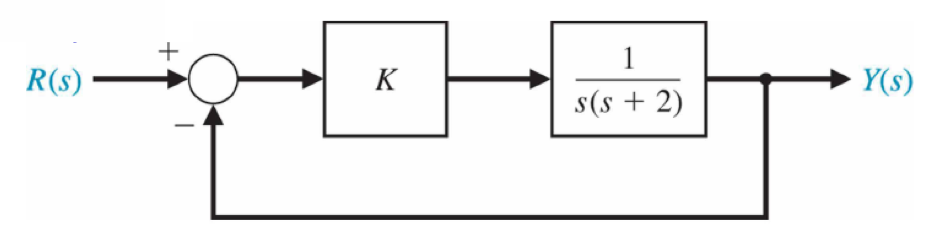
\includegraphics[width=0.8\linewidth]{./figures/2ordersys.png}
  \caption{Example 2nd order control system}
  \label{fig:2ordersys}
\end{figure}

In general, if the loop transfer function is
\begin{equation*}
  F(s) = K \frac{\prod_{i = 1}^{M} (s + z_i)}{\prod_{k = 1}^{n} (s + p_k)}
\end{equation*}
then the characteristic equation is
\begin{equation*}
  1 + F(s) = 0
\end{equation*}
and the root locus conditions become
\begin{align*}
  K \left| \frac{\prod (s + z_i)}{\prod (s + p_k)} \right| &= 1 \\
  \sum \angle (s + z_i) - \sum \angle (s + p_k) = \ang{180} + k \ang{360} 
.\end{align*}
So zeros add angle, whilst poles subtract angle.

\subsection{The Root Locus Procedure}
The following part will outline the general procedure for drawing a root-locus sketch.

\subsubsection{Prepare the Root Locus Sketch}
We should start by rewriting the characteristic equation so the gain appears as a multiplier
\begin{equation*}
  1 + KP(s) = 0
.\end{equation*}
Then factor $P(s)$ into poles and zeros.

The branches will always start at poles and end at zeros as
\begin{equation*}
  1 + K \frac{\prod (s + z_i)}{\prod ( s + p_k)} = 0
\end{equation*}
then, when $K = 0$ the equation reduces to the denominator being zero, so the roots are the open-loop poles, and when $K \to \infty$, the numerator dominates, so the roots approach the open-loop zeros.
So the root locus begins at poles and ends at zeros.
If there are fewer finite zeros than poles, then the extra branches go to zeros at infinity.
Also, because the coefficients are real, the locus is symmetri about the real axis.

\begin{exa}[Preparing the Locus sketch]
  We are given an example system
  \begin{equation*}
    1 + \frac{K}{s^{4} + 12s^3 + 64s^2 + 128s} = 0
  .\end{equation*}
  And we want to apply the above procedure to prepare a root locus sketch.
  \tcblower
  We factor the denominator:
  \begin{align*}
    s^{4} + 12s^3 + 64s^2 + 128 s &= s(s+4) \left( s^2 + 8s + 32 \right) \\
    &= s \left( s+4) \right) \left( s+4+4j \right) \left( s + 4 - 4j \right)
  .\end{align*}
  So the open loop poles are $s = 0, -4, -4 + 4j, -4-4j$, and there are no finite zeros.
  So the number of poles $n = 4$, the number of zeros $M = 0$, and the number of branches is 4.
\end{exa}

\subsubsection{Find the real-axis part of the locus}
We have a general rule stating that a point on the real axis is on the root locus if the number of poles and zeros to its right is odd.

For the above example, we have 0 singularities to the right of 0, so anything to the right of 0 is not on the locus.
Between $-4$ and 0, we have 1 singularity on the right so this part of the real axis is on the locus.
To the left of $-4$, we have 2 singularities to the right so this part of the real axis is not on the locus.
This means the only real-axis segment on the root locus is
\begin{equation*}
  -4 < s < 0
.\end{equation*}


\subsubsection{Asymptotes to Infinity}
Since there are more poles than zeros, some branches must go to infinity.
The number of asymptotes is
\begin{equation*}
  n - M = 4 - 0 = 4
.\end{equation*}

The asymptote angles are
\begin{equation*}
  \phi_A = \frac{(2k + 1) \ang{180} }{n - M}, \qquad k = 0,1,2,3
.\end{equation*}
So here:
\begin{equation*}
  \phi_A = \ang{45} , \ang{135} , \ang{225} , \ang{315} 
.\end{equation*}

The asymptote centroid is found as
\begin{equation*}
  \sigma_A = \frac{\sum \text{poles} - \sum \text{zeros}}{n - M}
.\end{equation*}
Here, the poles sum to $-12$ and the zeros sum to 0, so
\begin{equation*}
  \sigma_A = \frac{-12}{4} = -3
.\end{equation*}
So the four asymptotes all cross the real axis at $s = -3$, with angles $\ang{45} , \ang{135} , \ang{225} , \ang{315}$.

\subsubsection{Crossing Between Root Locus and the Imaginary Axis}
Here, we use the Routh-Hurwitz criterion.
We start by rewriting the characteristic equation as a polynomial:
\begin{equation*}
  s^{4} + 12 s^3 + 64s^2 + 128s + K = 0
.\end{equation*}
So our Routh array is
\begin{equation*}
  \begin{array}{c|cccc}
    s^{4} & 1 & 64 & K\\
  s^3 & 12 & 128 & 0\\
  s^2 & \frac{12 \cdot 64 - 1 \cdot 128}{12} & K & 0\\
  s^{1} & \frac{\frac{640}{12} \cdot 128 - 12K}{\frac{640}{12}} & 0 & 0\\
  s^{0} & K &  & \\
  \end{array}
.\end{equation*}
The $s^2$ row first term is $(768 - 128) / 12 = \num{53,33}$ and the $s^{1}$ ros first term becomes zero at the crossing 
\begin{equation*}
  \frac{\num{53,33} \cdot 128 - 12K}{\num{53,33}} = 0
\end{equation*}
which gives $K \approx \num{568,89}$.

Now we use
\begin{equation*}
  \num{53,33} s^2 + \num{568,89}  = 0
\end{equation*}
so $s^2 = \num{-10,67} \implies s \pm j \num{3,266}$.

So the root locus crosses the imaginary axis at $s \pm j \num{3,266}$ when $K = \num{568,89}$.

\subsubsection{Breakaway Points}
A breakaway point is where two branches meet on the real axis and then leave it into the complex plane.

Since the real-axis locus is only between $-4$ and 0, the poles at 0 and $-4$ move toward each other along that segment, meet, and then break away.

From
\begin{equation*}
  1 + \frac{K}{D(s)} = 0 \implies D(s) + K = 0 \implies K = -D(s)
\end{equation*}
where
\begin{equation*}
  D(s) = s(s+4)(s+4+4j)(s+4-4j)
.\end{equation*}
The breakaway points satisfy
\begin{equation*}
  \frac{\mathrm{d}K}{\mathrm{d}s} = 0
\end{equation*}
which is equivalent to differentiating $D(s)$.
The real solution on the locus is $s\approx \num{-1,577}$, so the branches from 0 and $-4$ meet around $s = \num{-1,577}$ and leave the real axis there. 

\subsubsection{Angle of departure from the complex poles}
Because there are complex poles at
\begin{equation*}
  -4 \pm 4j
\end{equation*}
the branches do not leave those poles in arbitrary directions.
They must satisfy the angle condition
\begin{equation*}
  \angle P(s) = (2k+1) \ang{180} 
.\end{equation*}
For the upper pole $-4 + 4j$, the angles contributed by the other poles are used to determine the departure angle.
We can find one equivalent angle as \ang{225}, and because angles are modulo \ang{360}, that is the same as \ang{-135}.
So the key-idea is that the departure direction is forced by the angle condition, and that the two complex-pole branches leave symmetrically. 

\subsubsection{Complete the Sketch}
Now all the pieces are known.
We have poles at 0, $-4$, and $-4\pm4j$, no finite zeros and the only part of the real axis on the locus is $(-4, 0)$. 
The asymptotes are through $-3$ at \ang{45} , \ang{135} , \ang{225} , and \ang{315}.
The breakaway is at \num{-1,577} and the imaginary crossing is at $\pm j \num{3,266}$ when $K = \num{568,89}$.

\subsection{Parameter Design by the Root Locus Method}
Suppose a system has a characteristic equation on the form
\begin{equation*}
  a_n s^{n} + a_{n-1}s^{n-1} + \ldots  + a_1 s + a_0 = 0
\end{equation*}
and we then want to know what happens when one coefficient, say $a_1$, changes.

We can rearrange the above into the root-locus form:
\begin{equation*}
  1 + \frac{a_1 s}{a_ns ^{n} + a_{n-1}s^{n-1} + \ldots  + a_2 s^2 + a_0} = 0
\end{equation*}
so now we can interpret it as a gain-like parameter $K = a_1$, and an open-loop part:
\begin{equation*}
  P(s) = \frac{s}{a_ns^{n} + a_{n-1}s^{n-1} + \ldots  + a_2 s^2 + a_0}
.\end{equation*}
So even though $a_1$ is not the loop gain, it can still be treated as the parameter that ``scales'' the transfer function.
Then the root locus tells us where the closed-loop poles go as $a_1 $ changes, whether stability improves or worsens, or how damping and speed change.

\subsubsection{Varying Multiple Parameters}
If we instead have a characteristic equation like
\begin{equation*}
  s^3 + s^2 + \beta s + \alpha = 0
\end{equation*}
and we want to adjust both the $\alpha$ and $\beta$ parameters, then we cannot directly make an ordinary root locus that simultaneously sweeps both $\alpha$ and $\beta$ as this method can only vary one scalar parameter at a time.
Instead we repeat the procedure twice.

We start by studying $\alpha$ by setting $\beta = 0$.
Then the characteristic equation becomes
\begin{equation*}
  s^3 + s^2 + \alpha = 0 \implies 1 + \frac{\alpha}{s^3 + s^2} = 0
.\end{equation*}
Now this is a root locus with parameter $K_2 = \alpha$ and tranfer function:
\begin{equation*}
  P_2 (s) = \frac{1}{s^3 + s^2}
.\end{equation*}
We then use this root locus to choose a useful value of $\alpha$ based on the pole locations we want.

Then we fix $\alpha$ at the chosen value and study $\beta$, by rewriting the equation as
\begin{equation*}
  1 + \frac{\beta s}{s^3 + s^2 + \alpha} = 0
\end{equation*}
so now the parameter is $K_1 = \beta$ and the transfer function is
\begin{equation*}
  P_1(s) = \frac{s}{s^3 + s^2 + \alpha}
.\end{equation*}
This, in turn, lets us see how the poles move as $\beta$ changes.
